\newpage
\section{FSM}

Beispiel:
\begin{figure}[htbp]
	\centering
	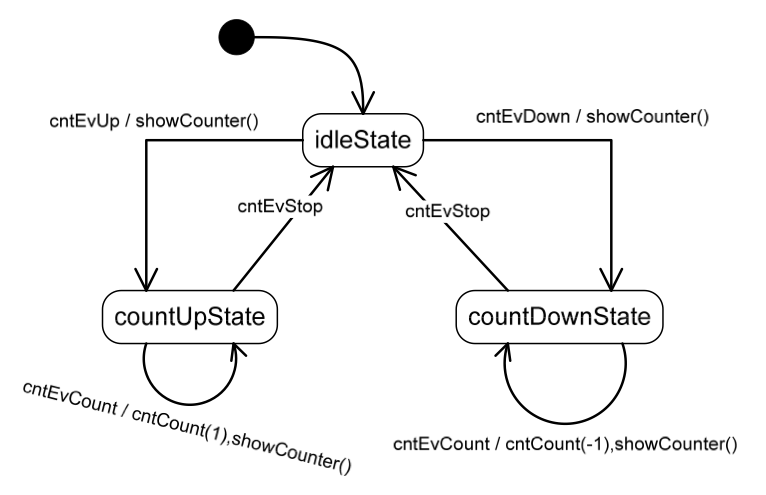
\includegraphics[width=9cm]{images/FSM.png}
\end{figure}

\subsection{Kontrollstrukturen in C }
\subsubsection{CounterCtrl.h}
\begin{lstlisting}[style=Csharp]
#ifndef COUNTERCTRL_H__
#define COUNTERCTRL_H__

typedef enum {cntEvUp,       // count upwards
              cntEvDown,     // count downwards
              cntEvCount,    // count (up or down)
              cntEvStop}     // stop counting
             CntEvent;

void cntCtrlInit();
// initializes counter FSM

void cntCtrlProcess(CntEvent e);
// changes the state of the FSM based on the event 'e'
// starts the actions

#endif
\end{lstlisting}

\subsubsection{CounterCtrl.c}
\begin{lstlisting}[style=Csharp]
#include <stdio.h>
#include "counterCtrl.h"
#include "counter.h"

typedef enum {idleState,        // idle state
              countUpState,     // counting up at each count event
              countDownState}   // counting down at each count event
             State;

static State currentState = idleState; // holds the current state of the FSM

void cntCtrlInit()
{
  currentState = idleState;
  cntInit(0);
}


void cntCtrlProcess(CntEvent e)
{
  switch (currentState)
  {
    case idleState:
      printf("State: idleState\n");
      if (cntEvUp == e)
      {
        // actions
        printf("State: idleState, counter = %d\n", cntGetCounter());
        // state transition
        printf("Changing to State: countUpState\n");
        currentState = countUpState;
      }
      if (cntEvDown == e)
      {
        // actions
        printf("State: idleState, counter = %d\n", cntGetCounter());
        // state transition
        printf("Changing to State: countDownState\n");
        currentState = countDownState;
      }
      break;
      
    case countUpState:
      printf("State: countUpState\n");
      if (cntEvCount == e)
      {
        // actions
        cntCount(1);
        printf("State: countUpState, counter = %d\n", cntGetCounter());
        // state transition
      }
      if (cntEvStop == e)
      {
        // actions
        // state transition
        printf("Changing to State: idleState\n");
        currentState = idleState;
      }
      break;
      
    case countDownState:
      printf("State: countDownState\n");
      if (cntEvCount == e)
      {
        // actions
        cntCount(-1);
        printf("State: countDownState, counter = %d\n", cntGetCounter());
        // state transition
      }
      if (cntEvStop == e)
      {
        // actions
        // state transition
        printf("Changing to State: idleState\n");
        currentState = idleState;
      }
      break; 
    default:
      break;
  }
}
\end{lstlisting}


\subsection{Kontrollstrukturen in C++}
\subsubsection{CounterCtrl.h}
\begin{lstlisting}[style=Csharp]
#ifndef COUNTERCTRL_H__
#define COUNTERCTRL_H__
#include "counter.h"

class CounterCtrl
{
  public:
    enum Event{evUp,       // count upwards
               evDown,     // count downwards
               evCount,    // count (up or down)
               evStop};    // stop counting
    CounterCtrl(int initValue = 0);
    void process(Event e);
    // changes the state of the FSM based on the event 'e'
    // starts the actions

  private:
    enum State{idleState,        // idle state
               countUpState,     // counting up at each count event
               countDownState};  // counting down at each count event

    State currentState;     // holds the current state of the FSM
    Counter myCounter;
};
#endif
\end{lstlisting}

\subsubsection{CounterCtrl.cpp}
\begin{lstlisting}[style=Csharp]
#include <iostream>
#include "counterCtrl.h"
#include "counter.h"
using namespace std;

CounterCtrl::CounterCtrl(int initValue) : 
  currentState(idleState),
  myCounter(initValue) { }

void CounterCtrl::process(Event e)
{
  switch (currentState)
  {
    case idleState:
      cout << "State: idleState" << endl;
      if (evUp == e)
      {
        // actions
        cout << "State: idleState, counter = " << myCounter.getCounter() << endl;
        // state transition
        cout << "Changing to State: countUpState" << endl;
        currentState = countUpState;
      }
      if (evDown == e)
      {
        // actions
        cout << "State: idleState, counter = " << myCounter.getCounter() << endl;
        // state transition
        cout << "Changing to State: countDownState" << endl;
        currentState = countDownState;
      }
      break;
      
    case countUpState:
      cout << "State: countUpState" << endl;
      if (evCount == e)
      {
        // actions
        myCounter.count(1);
        cout << "State: countUpState, counter = " << myCounter.getCounter() << endl;
        // state transition
      }
      if (evStop == e)
      {
        // actions
        // state transition
        cout << "Changing to State: idleState" << endl;
        currentState = idleState;
      }
      break;
      
    case countDownState:
      cout << "State: countDownState" << endl;
      if (evCount == e)
      {
        // actions
        myCounter.count(-1);
        cout << "State: countDownState, counter = " << myCounter.getCounter() << endl;
        // state transition
      }
      if (evStop == e)
      {
        // actions
        // state transition
        cout << "Changing to State: idleState" << endl;
        currentState = idleState;
      }
      break;
      
    default:
      break;
  }
}
\end{lstlisting}

\subsection{Tabelle}
\subsubsection{CounterCtrl.h}
\begin{lstlisting}[style=Csharp]
#ifndef COUNTERCTRL_H__
#define COUNTERCTRL_H__
#include "counter.h"

class CounterCtrl
{
  public:
    enum Event{evUp,       // count upwards
               evDown,     // count downwards
               evCount,    // count (up or down)
               evStop};    // stop counting
    CounterCtrl(int initValue = 0);
    void process(Event e);
    // changes the state of the FSM based on the event 'e'
    // starts the actions

  private:
    enum State{idleState,         // idle state
               countUpState,      // counting up at each count event
               countDownState};   // counting down at each count event

    State currentState;           // holds the current state of the FSM
    Counter myCounter;
    
    typedef bool (CounterCtrl::*Checker)(Event); // function ptr for checker function
    typedef void (CounterCtrl::*Action)(void);   // function ptr for action function
    // check functions
    bool checkIdleUp(Event check);
    bool checkIdleDown(Event check);
    bool checkUpIdle(Event check);
    bool checkDownIdle(Event check);
    bool checkUpUp(Event check);
    bool checkDownDown(Event check);
    
    // action functions
    void actionIdleUp(void);
    void actionIdleDown(void);
    void actionUpIdle(void);
    void actionDownIdle(void);
    void actionUpUp(void);
    void actionDownDown(void);
    
    struct Transition
    {
      State currentState;   // current state
      Checker pChecker;     // pointer to checker function
      Action pAction;       // pointer to action function
      State nextState;      // next state
    };
    static const Transition fsm[];
};
#endif
\end{lstlisting}

\subsubsection{CounterCtrl.cpp}
\begin{lstlisting}[style=Csharp]
#include <iostream>
#include "counterCtrl.h"
#include "counter.h"
using namespace std;

const CounterCtrl::Transition CounterCtrl::fsm[] =  // this table defines the fsm
{//currentState     checker function              action function               next state
  {idleState,       &CounterCtrl::checkIdleUp,    &CounterCtrl::actionIdleUp,   countUpState},
  {idleState,       &CounterCtrl::checkIdleDown,  &CounterCtrl::actionIdleDown, countDownState},
  {countUpState,    &CounterCtrl::checkUpUp,      &CounterCtrl::actionUpUp,     countUpState},
  {countUpState,    &CounterCtrl::checkUpIdle,    &CounterCtrl::actionUpIdle,   idleState},
  {countDownState,  &CounterCtrl::checkDownDown,  &CounterCtrl::actionDownDown, countDownState},
  {countDownState,  &CounterCtrl::checkDownIdle,  &CounterCtrl::actionDownIdle, idleState}
};

CounterCtrl::CounterCtrl(int initValue) : 
  currentState(idleState),
  myCounter(initValue)
{
}

void CounterCtrl::process(Event e)    // this function never changes
{
  for (unsigned int i = 0; i < sizeof(fsm) / sizeof(Transition); ++i) // determine number of transitions automatically
  {
    if (fsm[i].currentState == currentState &&  // is there an entry in the table?
        (this->*fsm[i].pChecker)(e))
    {
      (this->*fsm[i].pAction)();
      currentState = fsm[i].nextState;
      break;
    }
  }
}

// check functions
bool CounterCtrl::checkIdleUp(Event check)
{
  return evUp == check;
}

bool CounterCtrl::checkIdleDown(Event check)
{
  return evDown == check;
}

bool CounterCtrl::checkUpIdle(Event check)
{
  return evStop == check;
}

bool CounterCtrl::checkDownIdle(Event check)
{
  return evStop == check;
}

bool CounterCtrl::checkUpUp(Event check)
{
  return evCount == check;
}

bool CounterCtrl::checkDownDown(Event check)
{
  return evCount == check;
}

// action functions
void CounterCtrl::actionIdleUp(void)
{
  cout << "State: idleState, counter = " << myCounter.getCounter() << endl;
}

void CounterCtrl::actionIdleDown(void)
{
  cout << "State: idleState, counter = " << myCounter.getCounter() << endl;
}

void CounterCtrl::actionUpIdle(void)
{
}

void CounterCtrl::actionDownIdle(void)
{
}

void CounterCtrl::actionUpUp(void)
{
  myCounter.count(1);
  cout << "State: countUpState, counter = " << myCounter.getCounter() << endl;
}

void CounterCtrl::actionDownDown(void)
{
  myCounter.count(-1);
  cout << "State: countDownState, counter = " << myCounter.getCounter() << endl;
}
\end{lstlisting}

\subsection{State Pattern}
\subsubsection{CounterCtrl.h}
\begin{lstlisting}[style=Csharp]
#ifndef COUNTERCTRL_H__
#define COUNTERCTRL_H__
#include "counter.h"

class CounterState;  // forward declaration

class CounterCtrl
// this is the 'Context' class of the State pattern
{
  public:
    enum Event{evUp,       // count upwards
               evDown,     // count downwards
               evCount,    // count (up or down)
               evStop};    // stop counting
    CounterCtrl(int initValue = 0);
    void process(const Event e);  
    // changes the state of the FSM based on the event 'e'
    
  private:
    Counter counter;
    CounterState* pState;  // holds the current state
    friend class CounterState; // this (base) class is the only friend
};
#endif
\end{lstlisting}

\subsubsection{CounterCtrl.cpp}
\begin{lstlisting}[style=Csharp]
#include "counterCtrl.h"
#include "counterState.h"

CounterCtrl::CounterCtrl(int initValue): 
  counter(initValue), 
  pState(IdleState::getInstance()) // initial state
{
}

void CounterCtrl::process(const Event e)
{ // delegates all requests to CounterState
  pState =  pState->process(this, e);
}
\end{lstlisting}

\subsubsection{CounterState.h}
\begin{lstlisting}[style=Csharp]
#ifndef COUNTERSTATE_H__
#define COUNTERSTATE_H__
#include "counterctrl.h"  // Events are defined here

class CounterState  // virtual base class, not abstract!!
{
  public:
    virtual CounterState* process(CounterCtrl* pcontext, const CounterCtrl::Event e);
    // returns new state
  protected:    // only inherited classes may use these member functions
    CounterState* changeState(CounterCtrl* pcontext, CounterState* pnewState);
    Counter& myCounter(CounterCtrl* pcontext) {return pcontext->counter;}
};

class IdleState : public CounterState // it's a singleton
{
  public:
    static IdleState* getInstance();
    virtual CounterState*  process(CounterCtrl* pcontext, const CounterCtrl::Event e);
  private:
    IdleState() {};
    static IdleState instance;
};

class CountUpState : public CounterState // it's a singleton
{
  public:
    static CountUpState* getInstance();
    virtual CounterState*  process(CounterCtrl* pcontext, const CounterCtrl::Event e);
  private:
    CountUpState() {};
    static CountUpState instance;
};

class CountDownState : public CounterState // it's a singleton
{
  public:
    static CountDownState* getInstance();
    virtual CounterState*  process(CounterCtrl* pcontext, const CounterCtrl::Event e);
  private:
    CountDownState() {};
    static CountDownState instance;
};
#endif
\end{lstlisting}

\subsubsection{CounterState.cpp}
\begin{lstlisting}[style=Csharp]
#include <iostream>
#include "counterState.h"
using namespace std;


// class CounterState
CounterState* CounterState::process(CounterCtrl* pcontext, const CounterCtrl::Event e)
{
  return this;
}

CounterState* CounterState::changeState(CounterCtrl* pcontext, CounterState* pnewState)
{
  return pnewState;
}

// class IdleState
IdleState IdleState::instance;
IdleState* IdleState::getInstance()
{
  return &instance;
}

CounterState* IdleState::process(CounterCtrl* pcontext, const CounterCtrl::Event e)
{
  cout << "State: idleState" << endl;
  if (CounterCtrl::evUp == e)
  {
    // transition actions
    cout << "counter = " << myCounter(pcontext).getCounter() << endl;
    // state transition
    return changeState(pcontext, CountUpState::getInstance());
  }
  if (CounterCtrl::evDown == e)
  {
    // transition actions
    cout << "counter = " << myCounter(pcontext).getCounter() << endl;
    // state transition
    return changeState(pcontext, CountDownState::getInstance());
  }
  return this;
}

// class CountUpState
CountUpState CountUpState::instance;
CountUpState* CountUpState::getInstance()
{
  return &instance;
}

CounterState* CountUpState::process(CounterCtrl* pcontext, const CounterCtrl::Event e)
{
  cout << "State: countUpState" << endl;
  if (CounterCtrl::evCount == e)
  {
    // transition actions
    myCounter(pcontext).count(1);
    cout << "counter = " << myCounter(pcontext).getCounter() << endl;
    // state transition
    return changeState(pcontext, CountUpState::getInstance());
  }
  if (CounterCtrl::evStop == e)
  {
    // transition actions
    // state transition
    return changeState(pcontext, IdleState::getInstance());
  }
  return this;
}


// class CountDownState
CountDownState CountDownState::instance;
CountDownState* CountDownState::getInstance()
{
  return &instance;
}

CounterState* CountDownState::process(CounterCtrl* pcontext, const CounterCtrl::Event e)
{
  cout << "State: countDownState" << endl;
  if (CounterCtrl::evCount == e)
  {
    // transition actions
    myCounter(pcontext).count(-1);
    cout << "counter = " << myCounter(pcontext).getCounter() << endl;
    // state transition
    return changeState(pcontext, CountDownState::getInstance());
  }
  if (CounterCtrl::evStop == e)
  {
    // transition actions
    // state transition
    return changeState(pcontext, IdleState::getInstance());
  }
  return this;
}
\end{lstlisting}